%*******************************************************************************
%***********************************Tracking particles *****************************
%*******************************************************************************

\chapter[A Tracking Algorithm for Particle-like Objects]{A Tracking Algorithm for Particle-like Objects}
\label{ch:bacteria}
\dictum[Gottfried Leibniz]{There are two kinds of truths: those of reasoning and those of fact. The truths of reasoning are necessary and their opposite is impossible; the truths of fact are contingent and their opposites are possible.}%
\vskip 1em

\begin{flushright}\textit{This chapter is adapted from} \cite{dspataro:2017}.\end{flushright}
%\section{Introduction}
\lettrine[lines=3,lhang=0.33,lraise=0,loversize=0.15]{S}{tudying} the movement of sub-micron particles, micro-spheres and molecules under microscopic observation often requires their time trajectories from which important kinematic and dynamic properties can be computed. 
Several studies employ time-lapse microscopy, especially in the field of biophysics, as a tool to gather data and retrieve single particle time trajectories. The researcher usually relies on manual or semi-manual/interactive software to study such properties. However, this approach is unfeasible when the number of cells involved in the analysis is high.

In this Chapter  an original algorithm for detecting and tracking particles that is based on image processing techniques and to shape difference and centroid displacement analysis to reconstruct the trajectories is presented.
To our knowledge this is the first study regarding semi-automatic detection of particles-like objects adopting parallel CA.
In particular, the method works for $n$-dimensional input data provided that particles are represented by at least a centroid space coordinate and a geometrical entity which describe its shape. 
Since $2$D images are a common source of such data we also present framework for image-manipulation based on the Extended Cellular Automata(XCA) paradigm .

\texttt{TraCCA} has been successfully applied for the investigation of the motility of \textit{B. subtilis.} injected in a micro-fluidic device using 4100 images taken at 100 frames per second, as reported in Section \ref{sect:bacteriaanalysis}.

The Chapter is organized as follows: Sections  \ref{trackalgorithm} and \ref{manipulating} outline the proposed tracking algorithm and cellular automata based image processing framework, respectively; Section \ref{sect:bacteriaanalysis} shows a detailed application of \texttt{TraCCA} referred to a real case study regarding bacterial motility, while conclusions and possible future works are reported in Section \ref{conclusions}.


\section{Tracking Algorithm}\label{trackalgorithm}
The objective of the tracking algorithm is to produce a 
set $ T_n = \{ t_i \}$, where $t_i=\{ c^i_k,c^i_{k+1},\ldots,c^i_l \} $ 
of trajectories each described as a time-ordered list of positions in space from a set of input 
particles $P=P_1 \cup P_2 \cup \ldots \cup P_n$ and a function $\mathcal{D} :  P \times P \mapsto \mathbb{R}$, 
the \textit{distance} function. $P_i = \{p^j_i \; | \; 1 \leq j\; \}$ indicates all particles at time $i$ and each particle $p_i^j$ is defined by a centroid position, and a bounding box which describes its geometrical properties.
$\mathcal{D}(p,q)$ measures the likeliness that a particle $p$ has been transformed into $q$ as a result of the application of a number of geometrical transformations such as translation, scaling, shearing or rotation (see Eq. \ref{sec:bacttracking}). 
Indexes $k$ and $l$, $k \leq l$ indicate the trajectory starting and ending time of the tracked movement respectively, and the length $l-k+1$ is its duration in time.
Note that particles may appear or disappear at any time and hence $k\geq 0$ and $l \leq n$. Moreover, $|t_i| \leq l-k+1$ since a particle which has been successfully tracked
 from  $P_k$ to $P_{k^*} $ can disappear for a certain time and may appear again in $P_{\bar{k}}$, $k \leq k^* \leq \bar{k}$. We only allow disappearing time $\bar{k}-k^* \leq \xi$ where $\xi \geq 0$ is a parameter of the algorithm. 
Each trajectory  $t_*=\{ c^*_k,c^*_{k+1},\ldots,c^*_l \} $ is composed by  positions of particles $p^{j_1}_k,p^{j_2}_{k+1},\ldots,p^{j_*}_l$ at different times. 
This means that, for our purpose, particle $p^{j_1}_k$ at frame $k$ has moved from $c^*_k$ to location of particle $p^{j_2}_{k+1}$,$c^*_{k+1}$ at time ${k+1}$ and to location of $p^{j_*}_{l}$, $c^*_l$ at time $l$. 

As an example, let us consider a human tracking system where each $P_i$ could correspond to all the detected bodies in a  video frame $i$ and the distance function a linear combination of the euclidean distance between two detected bodies centroids  and pixel-by-pixel difference in colors of all the pixels within their bounding boxes. In this context, it would make sense to consider a not null disappearing time since it is not uncommon for the human detection module (which is in charge of producing the centroids and bounding box from the images) to skip recognizing a specific target only for a limited number of frames. 


In order to construct the trajectories, the algorithm works sequentially from frame $1$ to $n$ processing, at each step, two subsets of particles, $M_i$ and $P_{i}$, where $M_i$ contains all the corresponding trajectories ending particles $p^{j}_l$ that can still be expanded, i.e. $i-l \leq \xi$ .
Informally, the algorithm tries to augment an element in $M_i$ using a particle in $P_i$ making sure at most one particle is added to it, the same particle does not augment two different trajectories and the augmenting is performed s.t. the distance function is minimized.

Since at each step of the process a possible assignment between an element of $M_i$ and one of $P_i$ is sought, the algorithm can be thought to be similar to the \textit{assignment problem} \cite{bellmann1978} and more specifically, it consists in finding a minimum weight matching (not necessarily perfect) in  a weighted bipartite directed graph $G=(V,E)$ where $V={M_i} \cup P_i$ is the set of nodes and ${M_i}, P_i$ are the two partitions, $E = {M_i} \times P_i$ s.t. $e \in E, \mathcal{D}(e) \in \mathbb{R}$ is the weight of the edge.
A valid matching $S \subseteq E$ must satisfy the following: 
\begin{equation}
\forall (u,v) \in S 
\left\{
  \begin{array}{lr}
   (w,x) \in S,\; v=x\Longleftrightarrow u=w\\
   \mathcal{D}(u,v) = \min_{x \in V_2} \mathcal{D}(u,x)  \\
    \nexists \: (w,v) \in E \: \mbox{s.t.} \: \mathcal{D}(w,v) < \mathcal{D}(u,v)
  \end{array}
\right.
\label{matchConstraints}
\end{equation}

If we denote the matching operator  as the following recurrence relation $  M_i \lozenge P_{i+1} = (T_{i+1},M_{i+1}) $, $M_0=P_0$, then the  tracking algorithm can be summarized as $(T_n,M_n) = M_{n-1} \lozenge P_{n}=(((P_0 \lozenge P_1)\lozenge P_2) \lozenge \ldots \lozenge P_n)$.
If after the $\lozenge$ application a particle $p^* \in {M_i} \cup P_i $ remains  unmatched\footnote{$\nexists \;(u,v) \in S $ s.t. $  u=p^* \vee v=p^*$ (cf. Equation \ref{matchConstraints})}, two cases have to be considered (see Figure \ref{match}):
\begin{enumerate}
 \item if $p^* \in M_{i}$, the disappearing time counter $u_{p^*}$ for $p^*$ is updated and if $u_{p^*} > \xi$, $p^*$ is not included in $M_{i+1}$ and the corresponding tracked trajectory is flushed into $T_i$, otherwise it is retained. This handles the case when particles may disappear from the dataset for a number of time steps and appear again. 
 \item if $p^* \in P_i$, it corresponds to a newly appeared particle which is then inserted into $M_{i+1}$. 
\end{enumerate}
 
The pseudo-code reported in Algorithm \ref{matching} shows how the matching procedure is implemented. Note that the \texttt{NEIGH} procedure filters the possible candidates for a particle only to those which the euclidean spatial distance is less than a threshold parameter. In many real life applications particle displacement between two subsequent time-steps are small, so it would be useless trying to match a particle at time $i$ with one at time $i+1$ which are spatially far apart.

\begin{algorithm}[H]
    \SetKwInOut{Input}{Input}
    \SetKwInOut{Output}{Output}
   \underline{Function MATCH} $(M_i,P_{i+1})$\;
    \Input{Matched and to be matched particles $M$ and $P$ respectively.}
    \Output{$(T_{i+1},M_{i+1})$, which are the updated set of trajectories and matched particles.}
	
	$T_{i+1}=T_i$
    
    \ForEach{$p \in  M_i $}{
		 $neighbours[p] \gets NEIGH(p,P_{i+1})$	\;
		\ForEach{$n \in  neighbours[p]$}{
			 $d[p][n] \gets DISTANCE(p,n)$\;
		}
		 $SORTBY(neighbours[p],d[p])$\;
	}    
    


		\ForEach{ $p \in  M_i $}{
			
			\eIf {$neighbors[p].size \neq 0$}{
				 $\textit{candidate} \gets neighbors[p].first$
				}
				{
					$p.u \gets p.u+1$\;
					\textbf{continue}\;
				}
		
			\eIf {$match[candidate]=NIL$}
			{
				 $match[candidate] \gets p$\;
				 $p.u \gets 0$\;
			}
			{
				 $p' \gets match[candidate]$
					
		
				\eIf {$d[p][candidate] >= d[p'][candidate] $}{
					 $neighbors[p].pop()$
				}{
					 $\textit{match[candidate]} \gets p$\;
					 $neighbors[p'].pop()$ \;
					 $ p \gets p'$\;
				}
				\textbf{go to} $10$\;
			}
		}
    
 	\ForEach{$p \in  P_{i+1}$}{
		\eIf {$match[p]=NIL$}{
			 {$T_i+1.push(<p>)$}
		}{
			{
			$MATCH(T_{i+1},match[p]).enqueue(p))$}\;
		
			}
		}
		
	\ForEach{$p \in  M_{i} \cup P_{i+1}$}{
		\If {$p.u < P_r$}
			 {$M_{i+1}.push(p)$}
			
		}
		\Return $(T_{i+1},M_{i+1})$\;
    
    
      
 
    \caption{\texttt{TraCCA} tracking procedure}
		\label{matching}
\end{algorithm}


\definecolor{myblue}{RGB}{80,80,160}
\definecolor{mygreen}{RGB}{80,160,80}
\begin{figure}[!htb]
\centering
\begin{tikzpicture}[thick,
  every node/.style={draw,circle},
  fsnode/.style={fill=gray!30},
  ssnode/.style={fill=gray!90},
  every fit/.style={ellipse,inner sep=-2pt,text width=cm},
  ->,shorten >= 3pt,shorten <= 3pt
]

% the vertices of Frame1
\begin{scope}[start chain=going below,node distance=5mm, every node/.style={circle,minimum size=3.35em}]

\node[fsnode,on chain,label=above:$\boldsymbol{M_{i}}$] (f0)  {$p^i_1$};
\node[fsnode,on chain] (f1)  {$p^i_2$};

\node[below of=f1,node distance=10,yshift=-10] {$\vdots$};

\node[fsnode,on chain] (f2)  {$p^i_{j}$};
\node[below of=f2,node distance=10,yshift=-10] {$\vdots$};
\node[fsnode,on chain] (fl)  {$p^{i}_l$};
\node[below of=fl,node distance=10,yshift=-10] {$\vdots$};

\node[fsnode,on chain] (f3) {$p_n^i$};
\end{scope}

% the vertices of Frame1
\begin{scope}[xshift=6cm,start chain=going below,auto, every node/.style={circle,minimum size=3.3em},node distance=5mm]

\node[ssnode,on chain,label=above:$\boldsymbol{P_{i+1}}$] (s0)  {$p^{i+1}_1$};
\node[ssnode,on chain] (s1)  {$p^{i+1}_2$};
\node[draw=none,below of=s1,node distance=10,yshift=-10] {$\vdots$};

\node[ssnode,on chain] (sk)  {$p^{i+1}_k$};
\node[draw=none,below of=sk,node distance=10,yshift=-10] {$\vdots$};
\node[ssnode,on chain] (s2)  {$p^{i+1}_{m-1}$};
\node[ssnode,on chain] (s3)  {$p^{i+1}_m$};
\end{scope}
% the set U

\node [myblue,draw=none] {};
% the set V
\node [mygreen,draw=none] {};
  \begin{scope}[every edge/.style={draw,thin}]
% the edges
\draw (f0) edge[red, thick, dashed]  (s3);
\foreach \i in {0}
	\foreach \j in {0,1,2}
		\draw (f\i) edge  (s\j);


\draw (f1) edge[red,thick, dashed]  (s0);
\foreach \i in {1}
	\foreach \j in {1,2,3}
		\draw (f\i) edge  (s\j);

\draw (f2) edge[red, thick,dashed]  (s1);
\foreach \i in {2}
	\foreach \j in {0,2,3}
		\draw (f\i) edge  (s\j);

\draw (f3) edge[red, thick,dashed]  (s2);
\foreach \i in {3}
	\foreach \j in {1,3,0}
		\draw (f\i) edge  (s\j);
		
   \end{scope}



\end{tikzpicture}
\caption{An application of the $\lozenge$ operator referred to a frame $P_{i+1}$ of $m$ particles. Dashed red arrows highlight the solution $S$.
For instance, the trajectory $t_*=p^s_a \leadsto p^i_1$  is lengthened by $p^{i+1}_m$ becoming $t=p^s_a \leadsto p^i_1 \to p^{i+1}_m$.
Unmatching (no incident dashed red arrow are present) particle $p^{i+1}_k$  causes a  trajectory of length one to be created, while unmatching particle $p^{i}_l$ causes its disappearing time counter  to be updated and the corrensponding trajectory to be possibly finalized (if $u_{p^{i}_l} > \xi$). 
Note that, for the sake clarity, arrows for the unmatched  nodes are omitted.} \label{match}
\end{figure}

\section{Manipulating images using XCA}\label{manipulating}
In this section we present a Cellular Automata (\cite{Ilachinski2001,Neumann1966}) based framework for manipulating images that allows seamless parallel filters application.


\subsection{Definition and Usage}
The XCA adopted for manipulating images is defined as a $7$-tuple $ IFCA = \langle R,X,Q,P,\sigma,\Gamma,\gamma \rangle$ where:

    \begin{itemize}

    \item $R$ is the $2$-dimensional cellular space.

    \item $\Gamma \subseteq R$ is the region over where the global operation is applied

    \item $X=X(x_0,y_0)=\{(x,y): \left| x-x_0\right| \leq r \wedge \left| y-y_0\right| \leq r\} $ defines the \textit{Moore}'s neighborhood relationship of radius $r$

    \item $Q = Q_r \times Q_g \times Q_b \times Q_a$ representing the pixel color channels in the \texttt{RGBA} space.

    \item $P$ is the set of global parameters

    \item $\psi$ is the initialization function (which is in charge of reading images from files and converting them to substates).
      
    \item $\sigma=\{\sigma_i:Q^{|X|} \mapsto Q\}$ is the set of image convolutional filters (corresponding to XCA elementary processes)  

    \item $\gamma= \{\gamma_i:Q^{|\Gamma|} \rightarrow Q^{|\Gamma|}\} $ is the set of non-local filters (the XCA global functions).

    \end{itemize}
    
In order to take advantage of the intrinsic parallel nature of CA, \texttt{IFCA} is implemented augmenting an existing CA library, \texttt{\textbf{OpenCAL}} \cite{opencalurl} \cite{opencalmother} which is empowered  with a set of procedures that allows seamless input/output and image convolution.
More specifically each image is represented as an cellular automaton whose substates represent the color of the pixel and filters implemented as elementary processes composition (see listing \ref{list:imgman}). 

\lstset{language=[OpenCL]C,frame=tb,
	caption=Example of usage of the IFCA XCA engine. Lines 1-5 create a model and runtime for an image of size $IMG\_SIZE$ and dimension $DIM$. Lines 7 loads the image into the substate which, for the sake of brevity, is unique since the input image is assumed to be single channel. Lines 9-10 show the creation of two user defined filters and Lines 11-12 load them into the engine. The order in which they appear in the code specifies the order of execution that is triggered at line 14., 
	label=list:imgman, 
	basicstyle=\footnotesize\ttfamily,
	keywordstyle=\color{blue}\ttfamily,
	stringstyle=\color{red}\ttfamily,
	commentstyle=\color{green}\ttfamily,
	backgroundcolor=\color{light-gray}, 
	numbers=left,numbersep=3pt, 
	numberstyle=\tiny\ttfamily\color{gray}
	%	numberstyle=\tiny
}
\begin{lstlisting}
//Model and CA engine
CALMooreNeighborhood<DIM,RADIUS> neighbor;
MODELTYPE calmodel(IMG_SIZE,&neighbor,SPACE_FLAT);
CALRun calrun(&calmodel, 1, STEPS, UPDATE_IMPLICIT); 
CALSUBSTATE* bgr=calmodel.addSubstate<PIXELTYPE>();
//Image loading
bgr->loadSubstate(*(new std::function(loadImage<PIXELTYPE>)), "image.tiff");
//Image Filters Creations
ContrastStrchFlt<...>csf(bgr,1285,1542,0,65535,1);
ThresholdFlt<...> tf (bgr,0,61680,0,65535);
calmodel.addElementaryProcess(&cst);
calmodel.addElementaryProcess(&tf);
//Trigger execution
calrun->run();
\end{lstlisting}

\texttt{IFCA} is extensible as it allows the application of user-defined filters by only specifying the pixel transformation rules (or kernels in case of convolutional ones). 
Filters are then executed by the \texttt{IFCA} engine which comes with two parallel (\texttt{OpenMP} and \texttt{OpenCL})  and a serial implementations.
The parallel execution is completely transparent and automatic and may be extremely useful in such cases where the size of the image is large or filters are particularl



\section{Motility analysis of B. subtilis}
\label{sect:bacteriaanalysis}
\subsection{Introduction}

\begin{figure}
    \begin{minipage}{0.48\textwidth}
        \centering
        
\includegraphics[width=1.0\textwidth]{./images/bacteria/bacteriasmall}
        \caption{Raw input image. Bacteria appears as darker gray clusters, while light gray halos and white areas represent noise and PDMS chromatic aberrations.}\label{contrast}
    \end{minipage}
   % \hfill \\ % \hfill \\
    \begin{minipage}{0.48\textwidth}
        \centering
        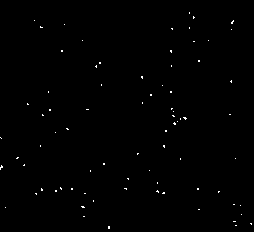
\includegraphics[width=1.0\textwidth]{./images/bacteria/bacteriasmall_threshold}
        \caption{Segmented and color inverted version of Figure \ref{contrast} as obtained by applying the filters (cf. Section \ref{Bacteriasegmentation}) using the IFCA model. White cluster of pixels represent bacteria.}\label{BBB}
    \end{minipage}
   
\end{figure}
In this section we present an application of \texttt{TraCCA} to the analysis of motion of \textit{B. subtilis.}
The analysis of trajectories in bacteria is really interesting because it is a non-invasive way of extracting much information about their chemotaxis which is the ability of bacteria to sense and respond to chemicals.
Thanks to chemotaxis, bacteria are able to reach a source of nutrient and move away from repellents, which makes it a key characteristic for their survival. Studying chemotaxis is really interesting not only because it has a strong influence on many biological mechanisms, e.g. biofilm formation and disease pathogenesis but also because  evolution's natural selection has optimized bacterial chemotaxis making bacteria excellent source-seekers and their strategies can be used to design bio-inspired, simple and efficient algorithms for robotic source locating systems. 
The motility  of \textit{B. subtilis} is composed of a series of \textit{run} (bacteria swim along smooth segments) and \textit{``tumbles''} (cells stop and randomly select a new direction).
Combining run and tumbles bacteria are able to direct their motility in order to reach nutrients and move away from repellent, in other words, to do their chemotaxis.
An algorithm that is able to track bacteria is really useful  because from bacterial trajectories much information about the way bacteria perform chemotaxis (e.g. duration of the run, swimming speed, frequency of tumbling events) can be extracted. 
This information is important in studying the strategy they adopt to reach a source of nutrient; moreover it is also interesting to investigating how the trajectories changes as certain environmental conditions change, such as temperature, oxygen concentration or gradient of chemicals.


In this work we used \textit{B. subtilis} strain \texttt{OI1085} for the tracking experiment.
Cells were taken from frozen stock, resuspended in CAM (Cap Assay Minimal) and shaken  (\SI{37}{\degree}, 100 rpm) until the optical density $OD600=0.3$ was reached; we then diluted the suspension 1:10 in CAM.
The bacterial suspension was injected in a micro-fluidic device.
The micro-fluidic device is a simple device made by \textit{PDMS} and glass, composed of three parallel channels (height  \SI{100}{\micro\meter}).
In the central channel (\SI{600}{\micro\meter} wide) bacteria were hosted and observed.
Two  walls of \textit{PDMS} (\SI{200}{\micro\metre}) separate the central channel from the left and right channels were oxygen was flown in order to reach a concentration of oxygen closed to 100\% in the central channel.
10 minutes after the injection of bacterial suspension a video was acquired at 100 frames per second for \SI{41}{\second}  (\#4100 frames). All images were acquired through a 10$\times$ phase contrast objective (\textit{Nikon} microscope), using binning $2 \times 2$.
All images are $512 \times 512$ pixels and have been exported in $16$-bit grayscale \texttt{TIFF} image format.

\subsection{Bacteria Segmentation}
\label{Bacteriasegmentation}

The \textit{B. subtilis} cells typically have a large range of motion patterns and the cell soma generally appears as a dark area surrounded with a white halo.
Colors can be inverted and the cell may appear white when it  moves out of focus sufficiently (see Figure \ref{contrast}).
In order to automatically detect \textit{subtilis} cells, it is possible to use a histogram-based thresholding method as suggested in \cite{Cho:1989}.
A key step of tracking bacteria is to individuate first, and then to label and describe each of the bacteria present in the images.
For this purpose,  a segmentation preprocessing phase is performed on all the images. 
Segmentation  is carried out by means of a threshold method \cite{Shapiro:2002} which produces a bipartition of pixels based on the color intensity. The value of pixel $(x,y)$ in image $g$ is given by the following, where $P$ is a predicate and $f$ is the original image:
\[{g(x,y) = \begin{cases} 1, & \mbox{if } P(f(x,y),T) \\ 0, & \mbox{otherwise }\end{cases}}\]
As a consequence, a drawback of using the threshold method is that, among all inter-pixels relationships, color intensity difference is the only involved by the bi-partition process.
This can easily lead to binary regions where pixels are not contiguous or to miss or include relevant or unwanted pixels respectively, with these effects getting worse as the noise increases.
In the considered case, however, the threshold method works well because after the application of the \texttt{contrast stretch filter} the analysed images present high contrast between the background and cells soma (see Figure \ref{contrast}), since the filter stretches or scales the range of pixel values between an upper and lower limit.
More specifically, color values that are above or below this range are saturated to the upper or lower limit values respectively, while values that lay in the interval are scaled according to the following formula: 
\[{g(x,y) = \begin{cases} L_o & \mbox{if } f(x,y) < L_i \\  H_o & \mbox{if } f(x,y) > H_i\\ L_o + (f(x,y)-L_i)\frac{H_o-L_o}{H_i-L_i} & \mbox{if } L_i \leq f(x,y) \leq H_i\end{cases}}\] where  $[L_i,H_i]$ defines the interval in the original image which is linearly scaled into the interval $[L_o,H_o]$.

Eventually, all the images go through a noise reduction stage which employs a combinations of \textit{gaussian}, \textit{laplacian} and \textit{blurring} filters \cite{Deng:1993}.
It is worth to note that filters parameters are dataset dependent and the best set of values experimentally determined. 
    \begin{figure}
    	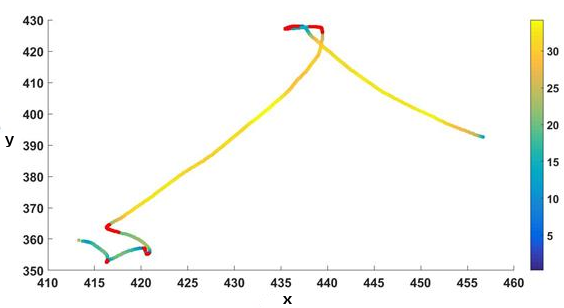
\includegraphics[width=0.6\textwidth]{./images/bacteria/runtumble.png}
    	\caption{An example of tracked trajectory of a single bacterium. Blue-yellow colors levels are proportional to the velocity, while dark red segments represent the individuated tumbles.}
    	\label{runtumbledetection}
    \end{figure}


\subsection{Bacteria Tracking}

Binary images are then used to extract the relevant information (shape and centroid) for each of the segmented bacteria.
This is done by interpreting each image as a graph whose nodes are pixels and arc $(i,j)$ exists if pixels $i$ and $j$ are neighbours (according to \textit{Moore}'s relationship, see section \ref{ch:CA}).
A bacterium corresponds to a connected component that can be easily individuated by using the DFS visiting algorithm.
Once all pixels that make up the cell soma are individuated, a unique \textit{ID} $id_i$ which identifies the bacterium uniquely, a centroid $c_i$ and a bounding box $s_i$ which describe the location, the shape and the area, respectively, are computed for each bacterium $i$. All the bacteria whose extension is less than $M_e = 2$\textit{px} are ignored and no further considered.
The creation and manipulation of all the geometrical entities involved in this latter phase are carried out by means of the computational geometry library \texttt{CGAL}  \cite{CGAL}.

In order for the application of the algorithm described in Section \ref{trackalgorithm}, a distance function is required.
Among possible functions, a linear combination of the centroids displacement and shapes difference was adopted:
\begin{equation}
\label{sec:bacttracking}
D(c_i,c_j) = a \sqrt{(x_{c_i} - x_{c_j})^2 + (y_{c_i}-y_{c_j})^2} + b |S_i \cap S_j|
\end{equation}
where $S_i$ and $S_j$ are the sets of pixels within the boundaries of the bacteria's  bounding box. Best values of weights $a$ and $b$ were experimentally determined in being $0.6$ and $0.4$ respectively. 
%REVIEW
Parameters search is carried out by computing the confusion matrix for 5 randomly picked images and for different values of $a,b \in \{\frac{i}{20}\;|\;0\leq i \leq 20\}$ and then choosing the ones minimizing false negatives and false positives and maximizing true negatives and true positive ones. 

Figure \ref{4traj} shows 4 snapshots of the outcome of the tracking algorithm for 4 bacteria taken at 4 different times, while Figure \ref{result} depicts the final collective view of all bacteria movements in the considered case study. 


\subsection{Analysis and Validation}
Starting from the relationship $D_b=  \frac{v^2 t_t}{2}$  \cite{Berg:1993} that links the diffusion coefficient to both swim velocity ($v$) and tumbling time ($tt$), 
we have partitioned each trajectory into running and tumbling events. 
These events allow the swimming speed to be calculated as difference between subsequent bacteria positions and average tumbling time as the overall time spent tumbling over by the number of tumbling events. 
Inspired by the work of \textit{Wong-Ng et al.} \cite{Wong2016} and \textit{B. Masson et al.} \cite{Masson:2011} an algorithm, implemented in \textit{MATLAB}, was adopted for detecting such running/tumbling events (see Figure \ref{runtumbledetection})  which in turn were used to extract all the relevant bacterial motility parameters from the tracked trajectories\footnote{Tumbles are associated both to a decrease in advancing velocity and an abrupt change in the angular velocity (i.e. in the direction of the motion). By fixing a threshold on both advancing and angular velocities it is possible to identify running/tumbling and use them to compute the mean values $t_t$ and $v$ over all the trajectories of the experiment.}.

The main parameters that were considered as as descriptors of the motion of the bacteria were: 
\begin{itemize}
\item \textit{Mean Swimming Velocity} ($\overline{v}$),
\item \textit{Mean Run Time} ($\overline{r_t}$) and 
\item \textit{Tumble Time} ($\overline{t_t}$).
\end{itemize}
By analyzing the entire trajectory set produced by \texttt{TraCCA} on the dataset described in Section \ref{sec:bacttracking}, the obtained values of the motion descriptors  were the following: 
\begin{itemize}
\item $\overline{v}$ =\SI{18}{\micro\meter \per \second},
\item $\overline{rt}$ = \SI{0.8}{\second}
\item $\overline{t_t}$= \SI{0.18}{\second}.
\end{itemize}
These experimental values\footnote{These motility parameters were also calculated using the \textit{Mean Square Displacement} (\texttt{MSD}) in time (which for the sake of brevity is only outlined here) by means of the MATLAB \texttt{@msdanalyzer} implementation \cite{msdanalyzer} and considering the following relationship $MSD(t)=\frac{1}{2}\frac{v^2 t_R^2}{2t/t_R +e^{\frac{-2t}{t_R}-1}}$ \cite{Howse2007} where $v$ is the swimming speed, $t_R$ is the timescale associated to rotational diffusion that is $t_R=2t_t$, it is possible to obtain $t_R $ and $v$ via fitting. $t_t$ and $v$ are then used to compute $D_b$.} are in accordance with those available in the literature as for instance in the work of \textit{Cisneros et al.} \cite{Cisneros:2011}.
\begin{figure}
	\begin{center}
		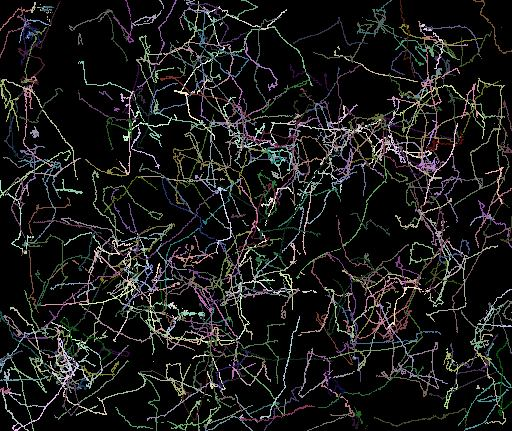
\includegraphics[width=0.85\textwidth]{./images/bacteria/result.png}
		\caption{Final collective view of all the tracked bacteria tracjectories as obtained by processing all 4100 images of the case study dataset. For the sake of figure clarity, a random color is associated to each bacterium trajectory.}\label{result}
	\end{center}
\end{figure}

\section{Conclusion}\label{conclusions}
In this preliminary work, a cellular-automata based tracking framework composed by a tracking algorithm and a CA support model for image processing, is presented for reconstructing trajectories of particle-like objects. This work reports the application to a real case study concerning the tracking of \textit{B. subtilis}, by evaluating  standard motility parameters (average swimming velocity, running and tumble times) in a microfluidic device. Results that were obtained during experimentation, proved that the \texttt{TraCCA} framework has correctly reconstructed bacterial trajectories. The tracking algorithm described in this work can also be effectively adopted in other fields as, for instance, crowd dynamics, provided that traceable elements can be described by means of a bounding box and a position.
\begin{figure}
	\setlength{\tabcolsep}{-0.02cm}
	\begin{tabular}{cccc}
		\subfloat{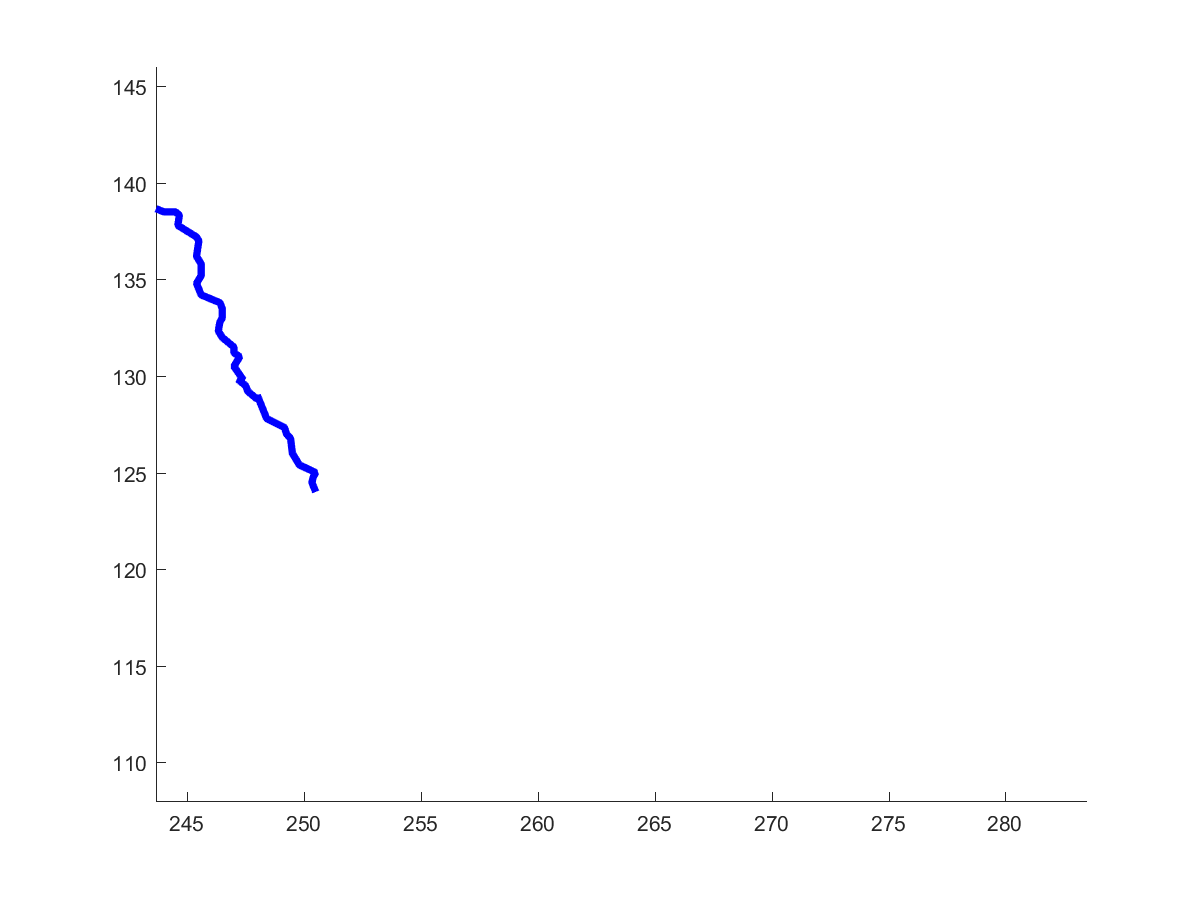
\includegraphics[width=0.25\textwidth]{./images/bacteria/1.png}} &
		\subfloat{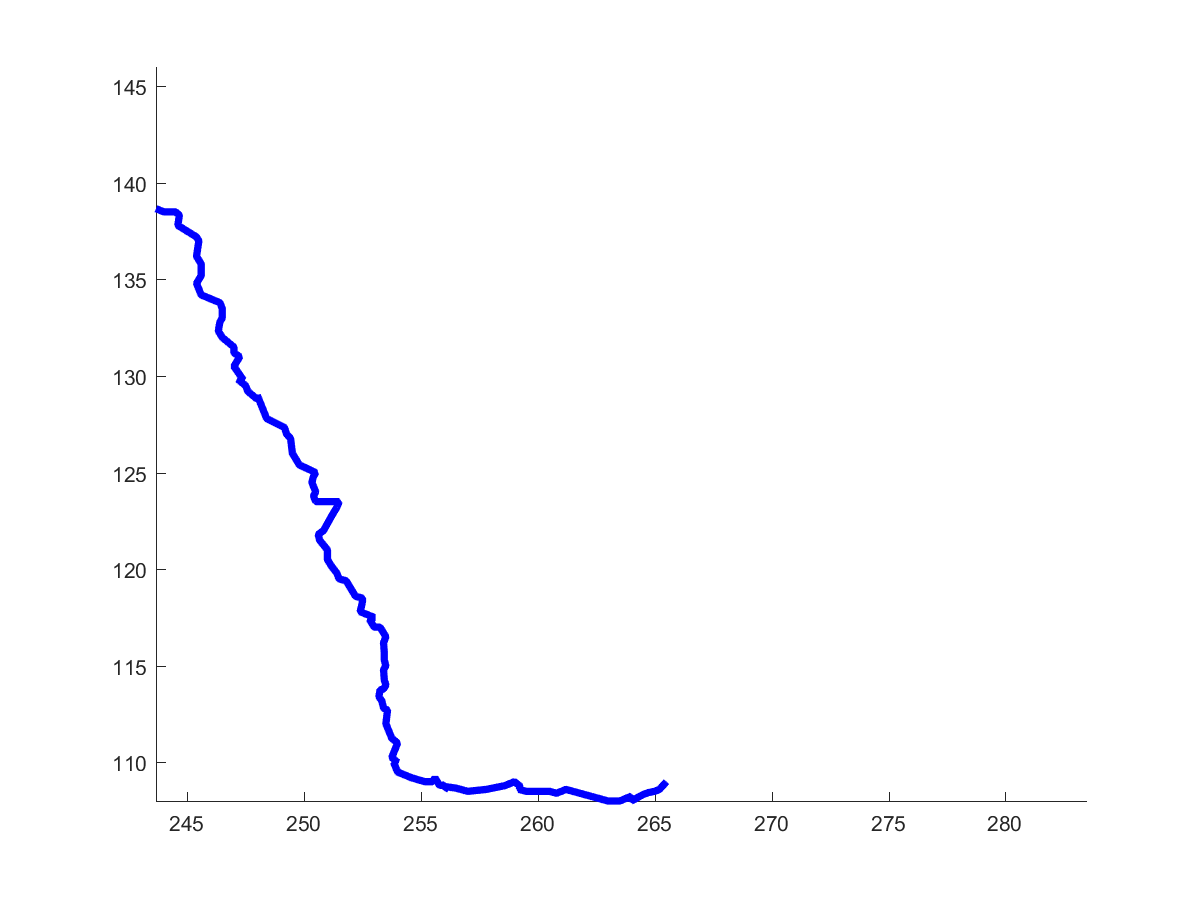
\includegraphics[width = 0.25\textwidth]{./images/bacteria/2.png}} &
		\subfloat {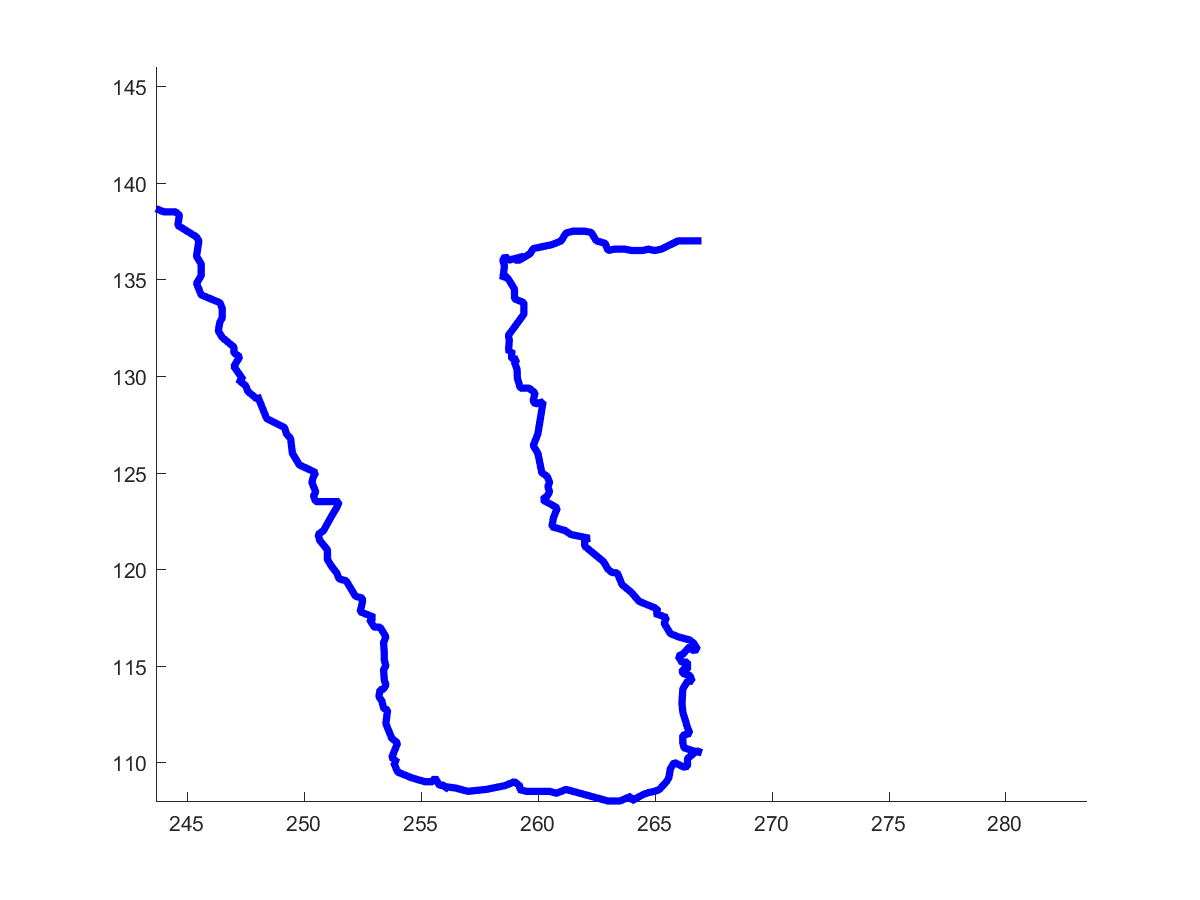
\includegraphics[width = 0.25\textwidth]{./images/bacteria/3.png}} &
		\subfloat {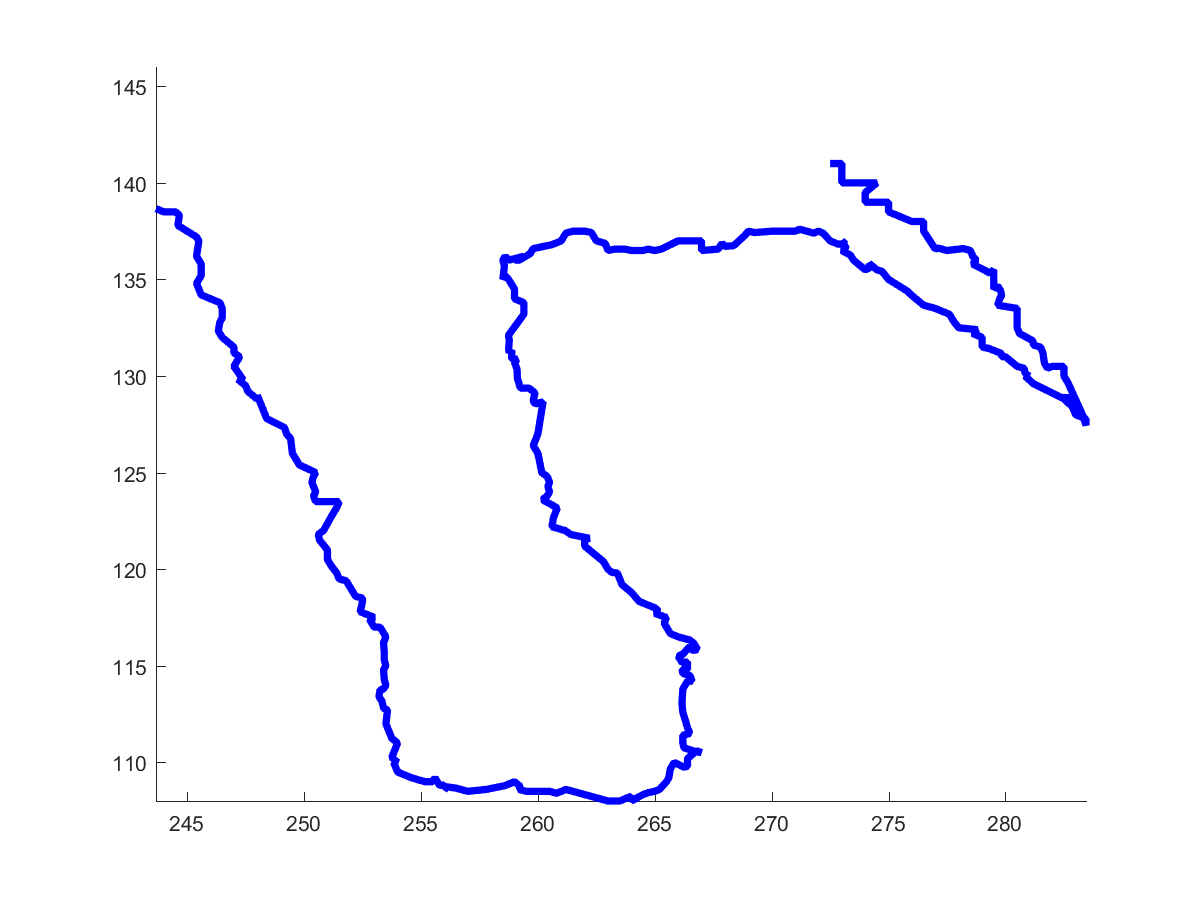
\includegraphics[width = 0.25\textwidth]{./images/bacteria/4.png}}\\
		\subfloat{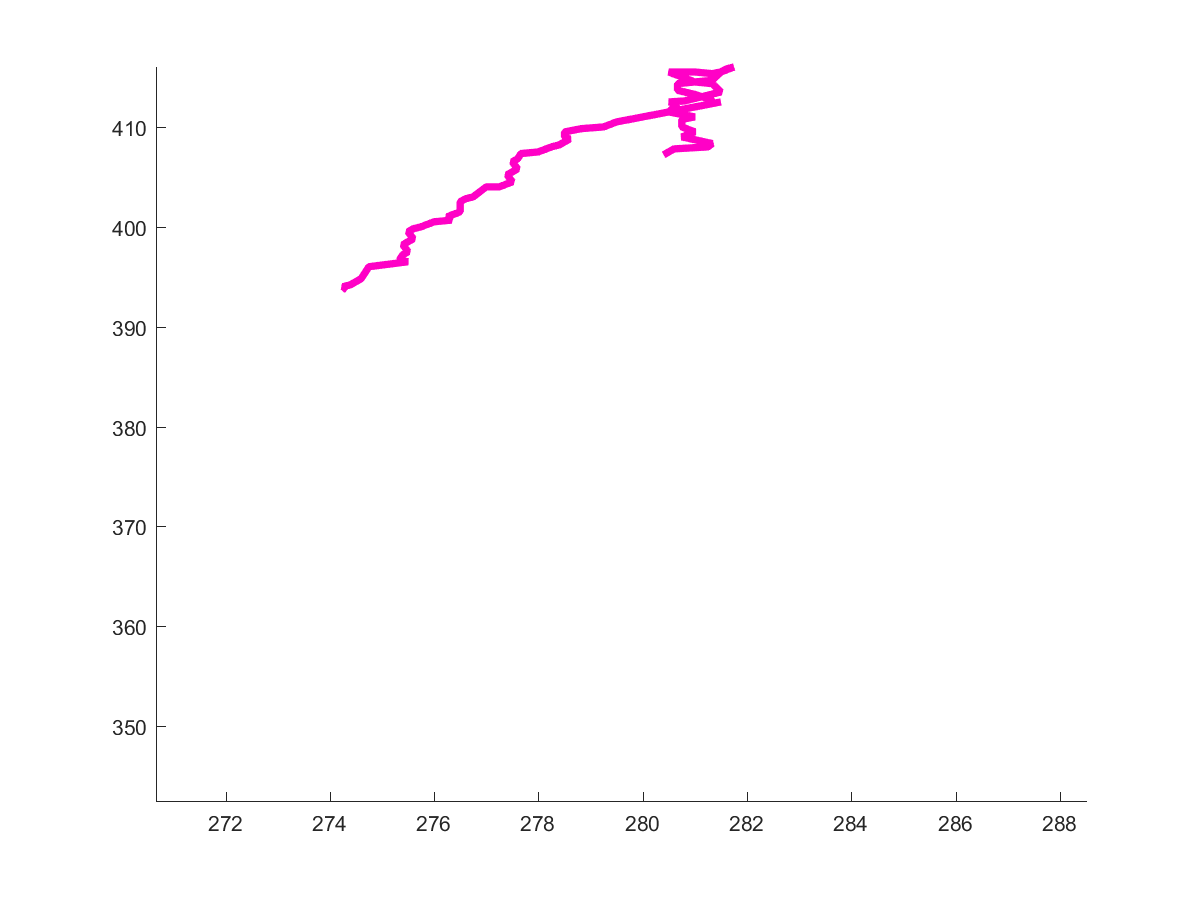
\includegraphics[width = 0.25\textwidth]{./images/bacteria/5.png}} &
		\subfloat {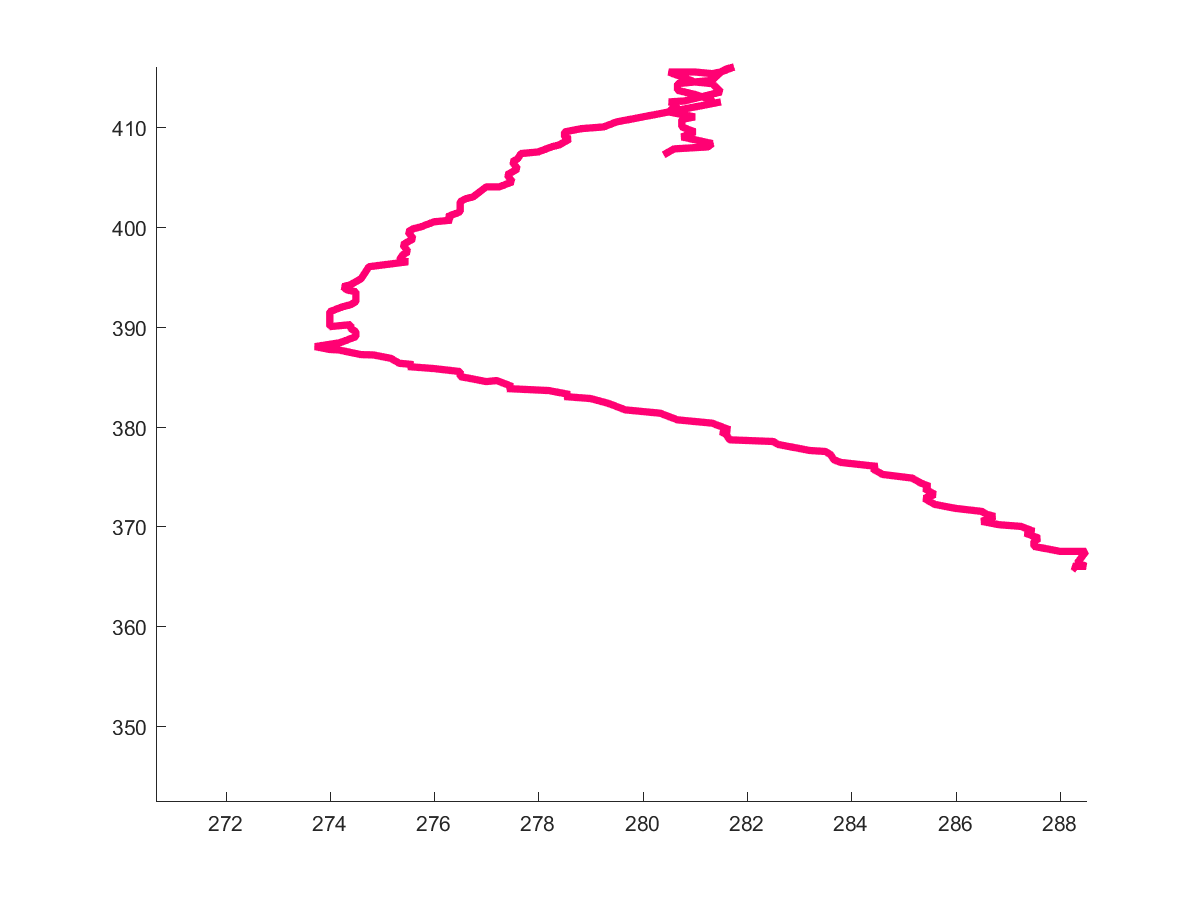
\includegraphics[width = 0.25\textwidth]{./images/bacteria/6.png}} &
		\subfloat {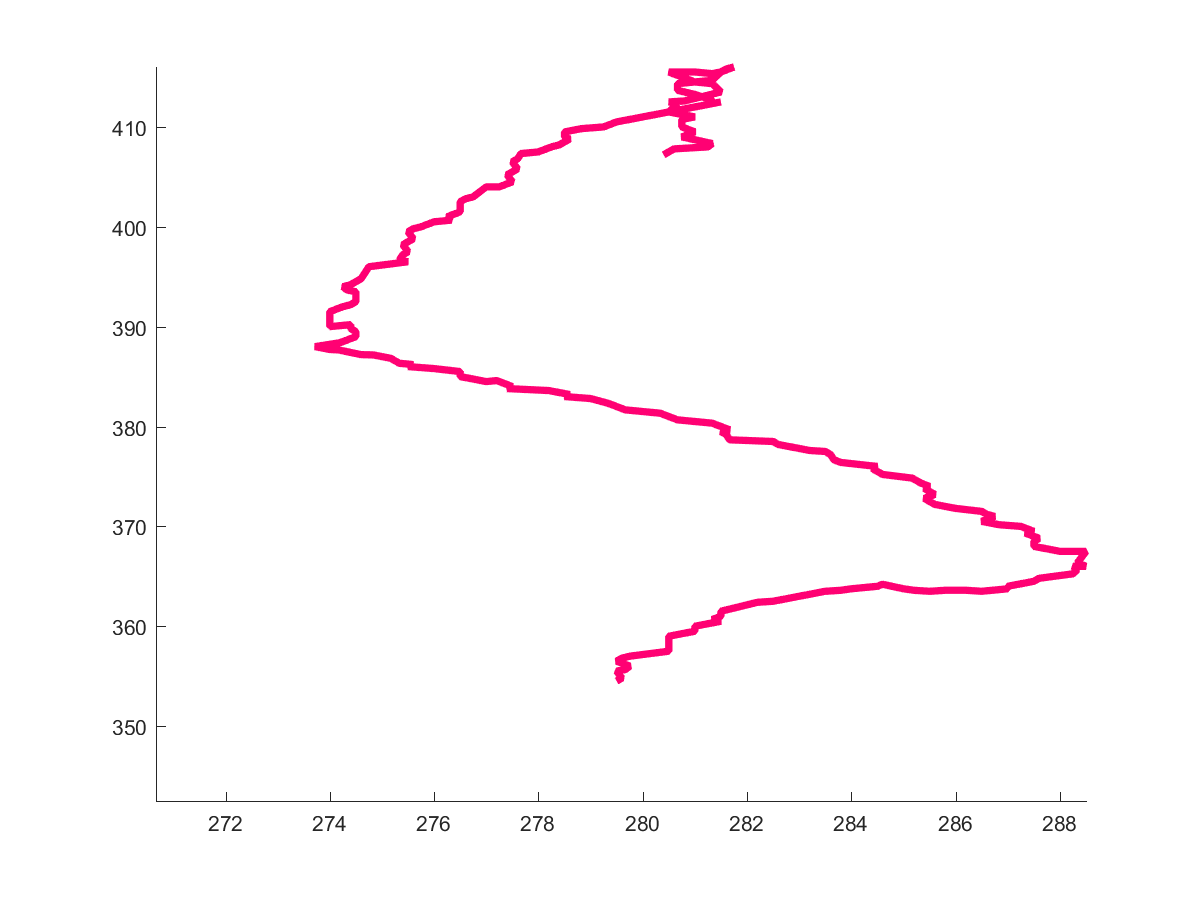
\includegraphics[width = 0.25\textwidth]{./images/bacteria/7.png}} &
		\subfloat {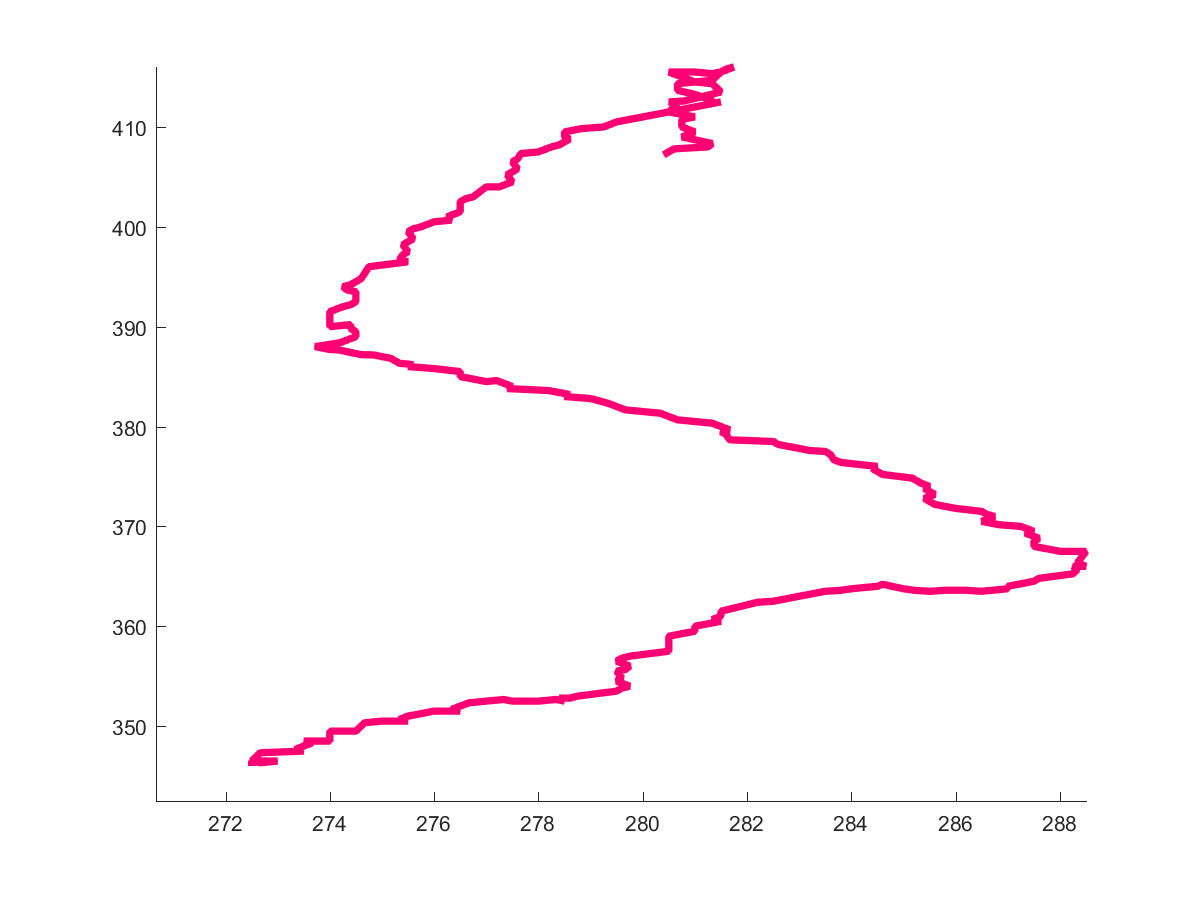
\includegraphics[width = 0.25\textwidth]{./images/bacteria/8.png}}\\
		\subfloat{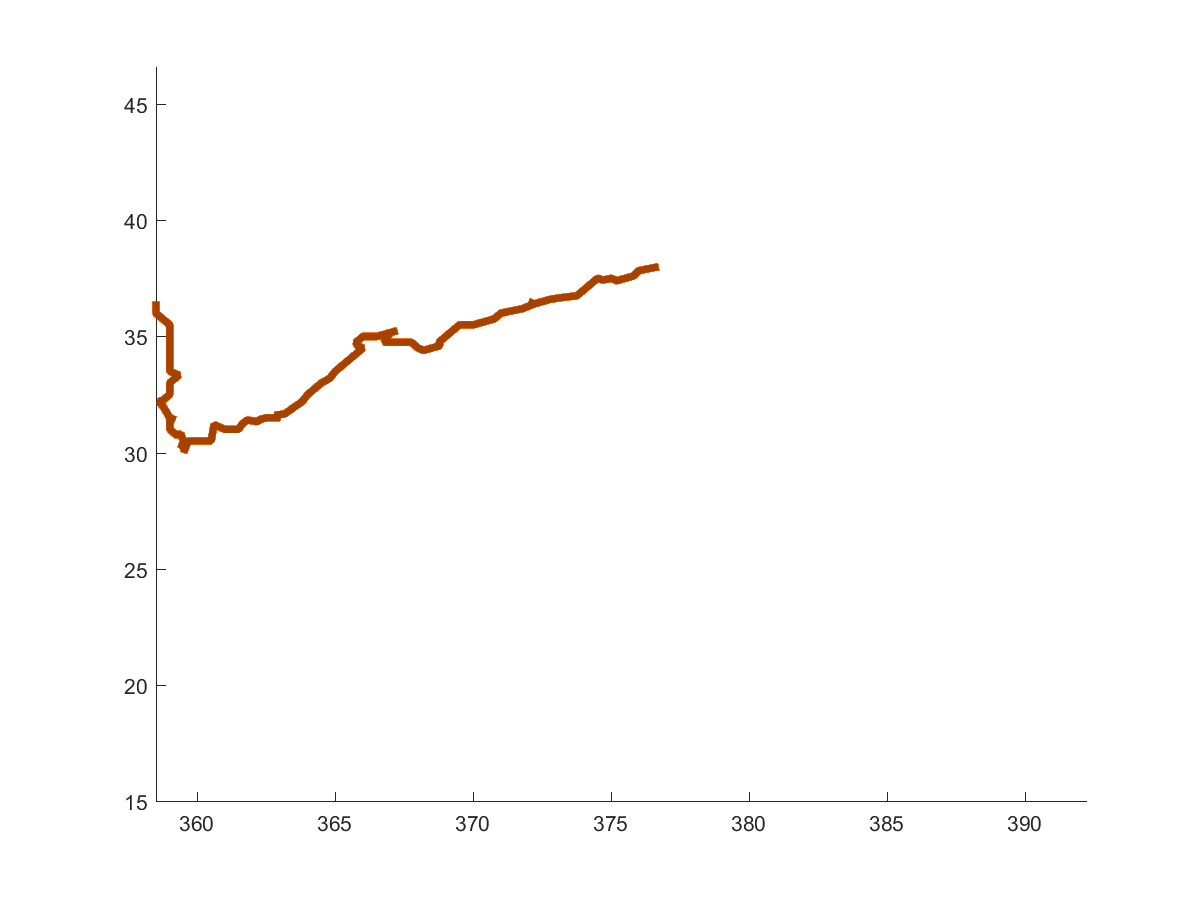
\includegraphics[width = 0.25\textwidth]{./images/bacteria/9.png}} &
		\subfloat {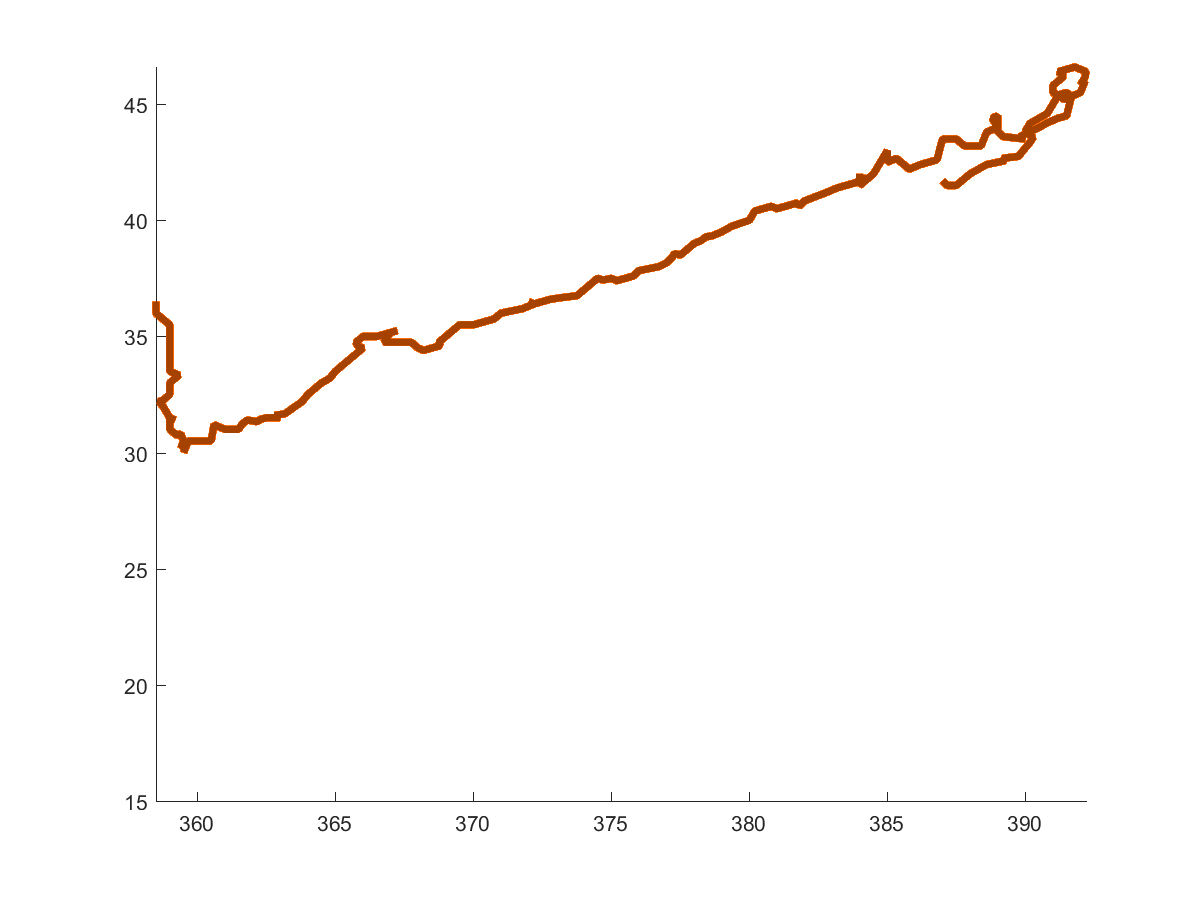
\includegraphics[width = 0.25\textwidth]{./images/bacteria/10.png}} &
		\subfloat {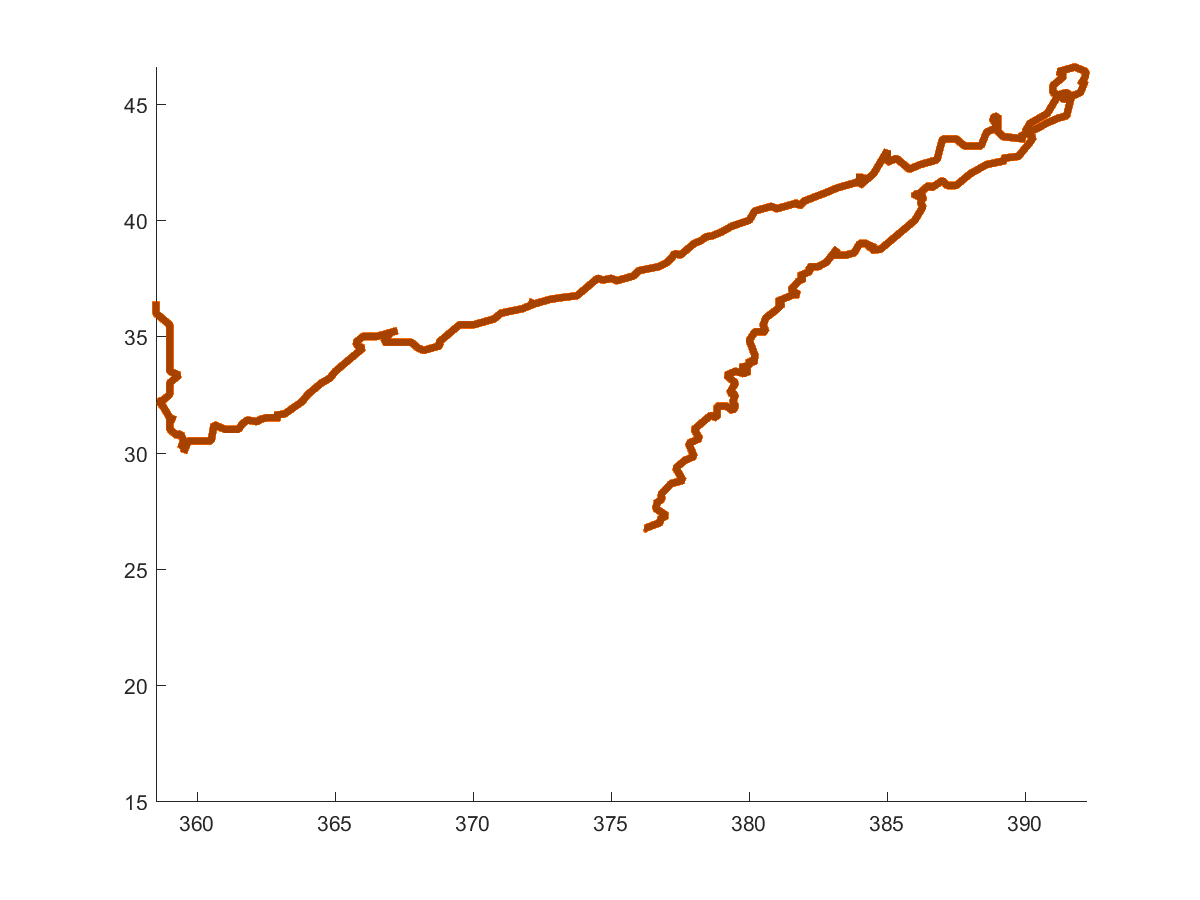
\includegraphics[width = 0.25\textwidth]{./images/bacteria/11.png}} &
		\subfloat {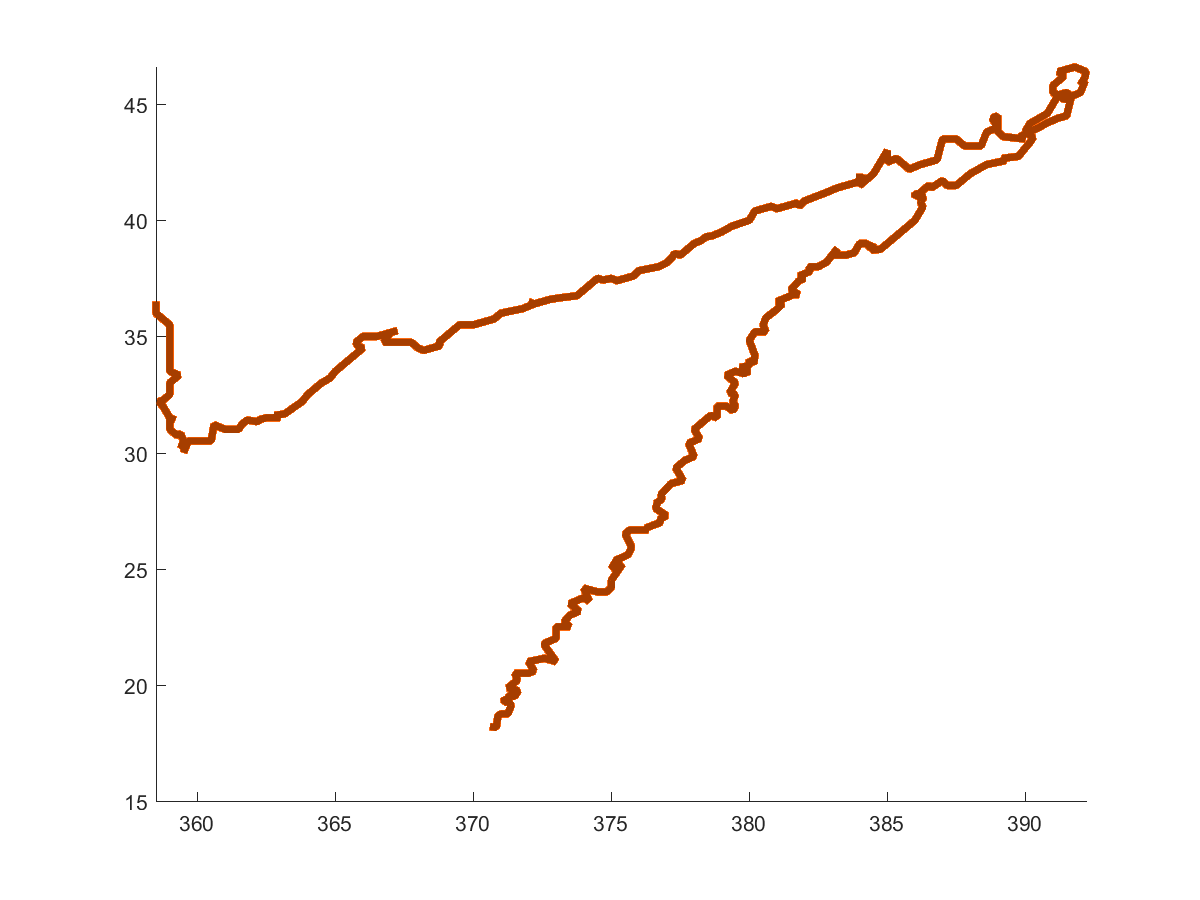
\includegraphics[width = 0.25\textwidth]{./images/bacteria/12.png}}\\
		\subfloat{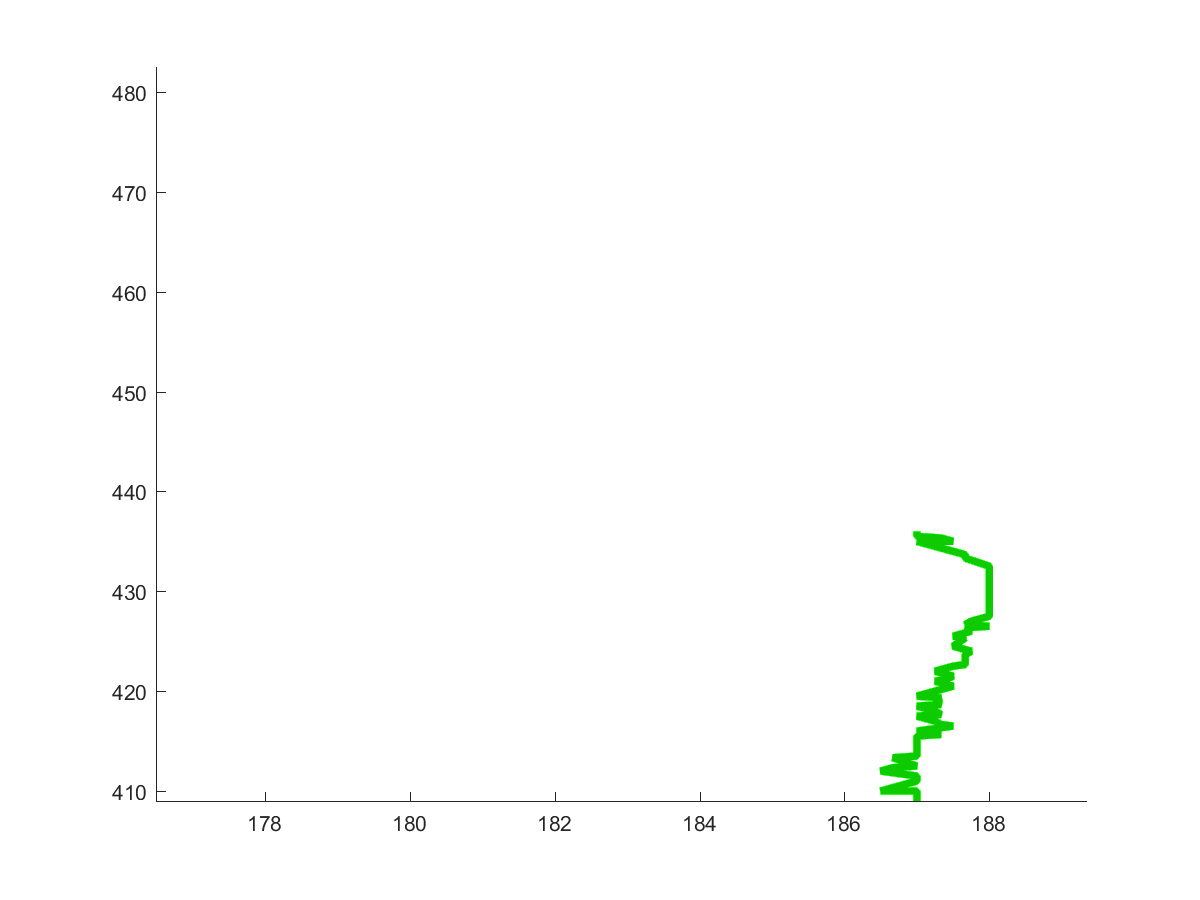
\includegraphics[width = 0.25\textwidth]{./images/bacteria/13.png}} &
		\subfloat {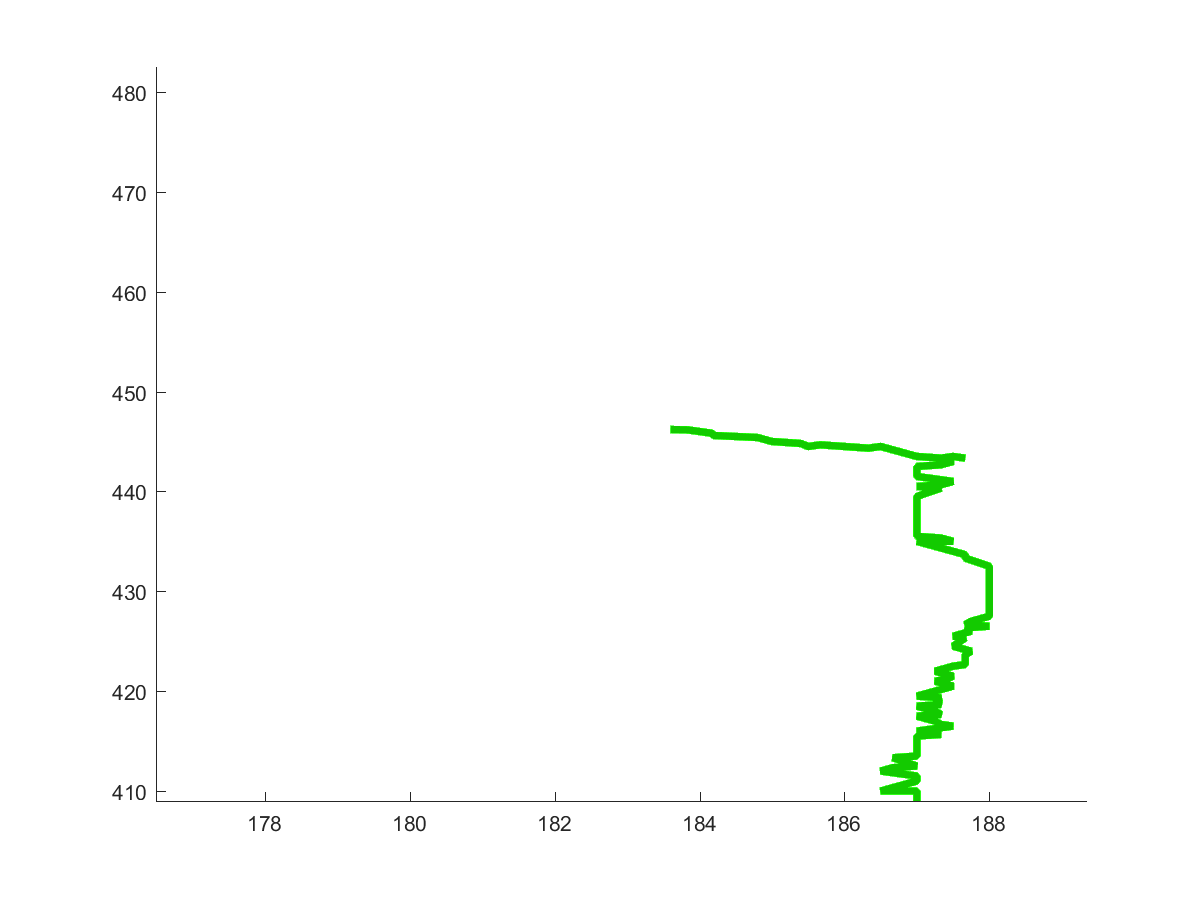
\includegraphics[width = 0.25\textwidth]{./images/bacteria/14.png}} &
		\subfloat {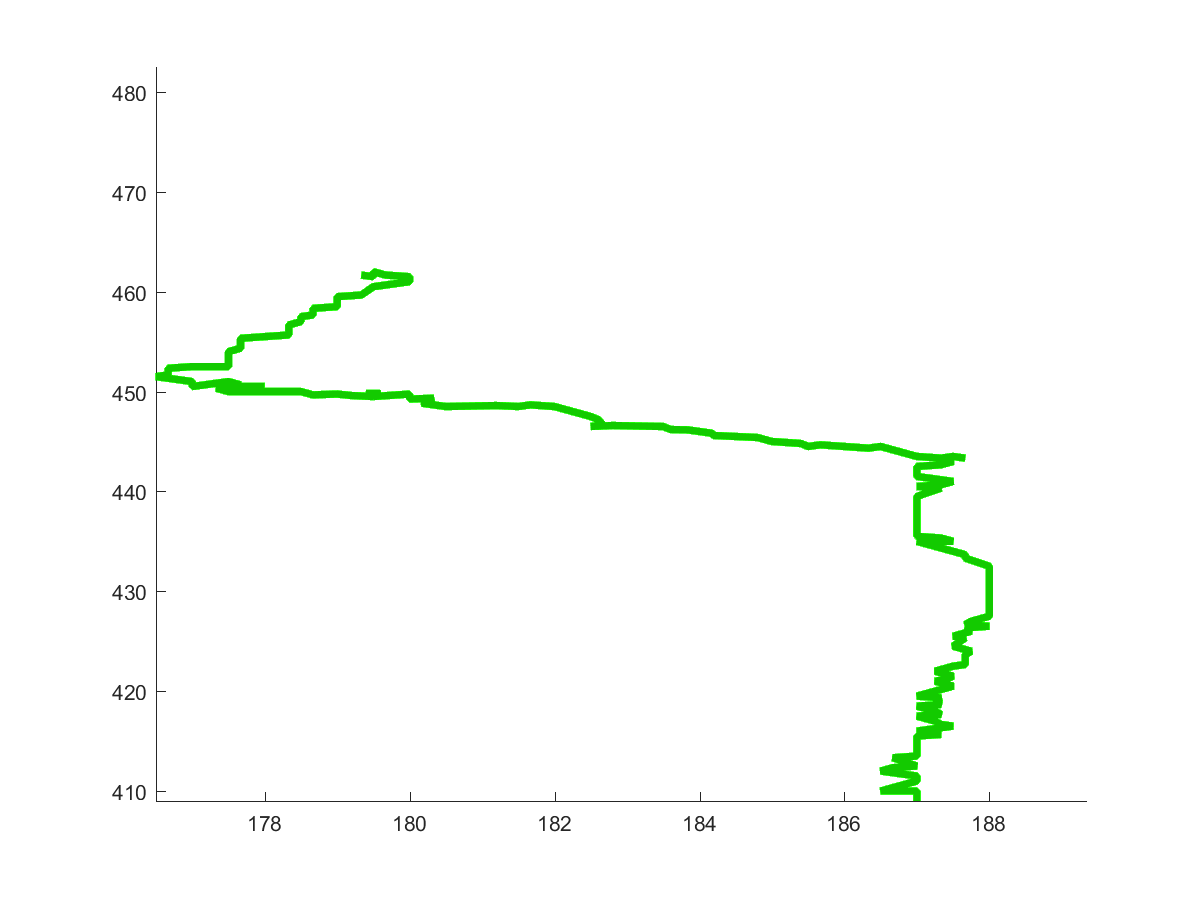
\includegraphics[width = 0.25\textwidth]{./images/bacteria/15.png}} &
		\subfloat {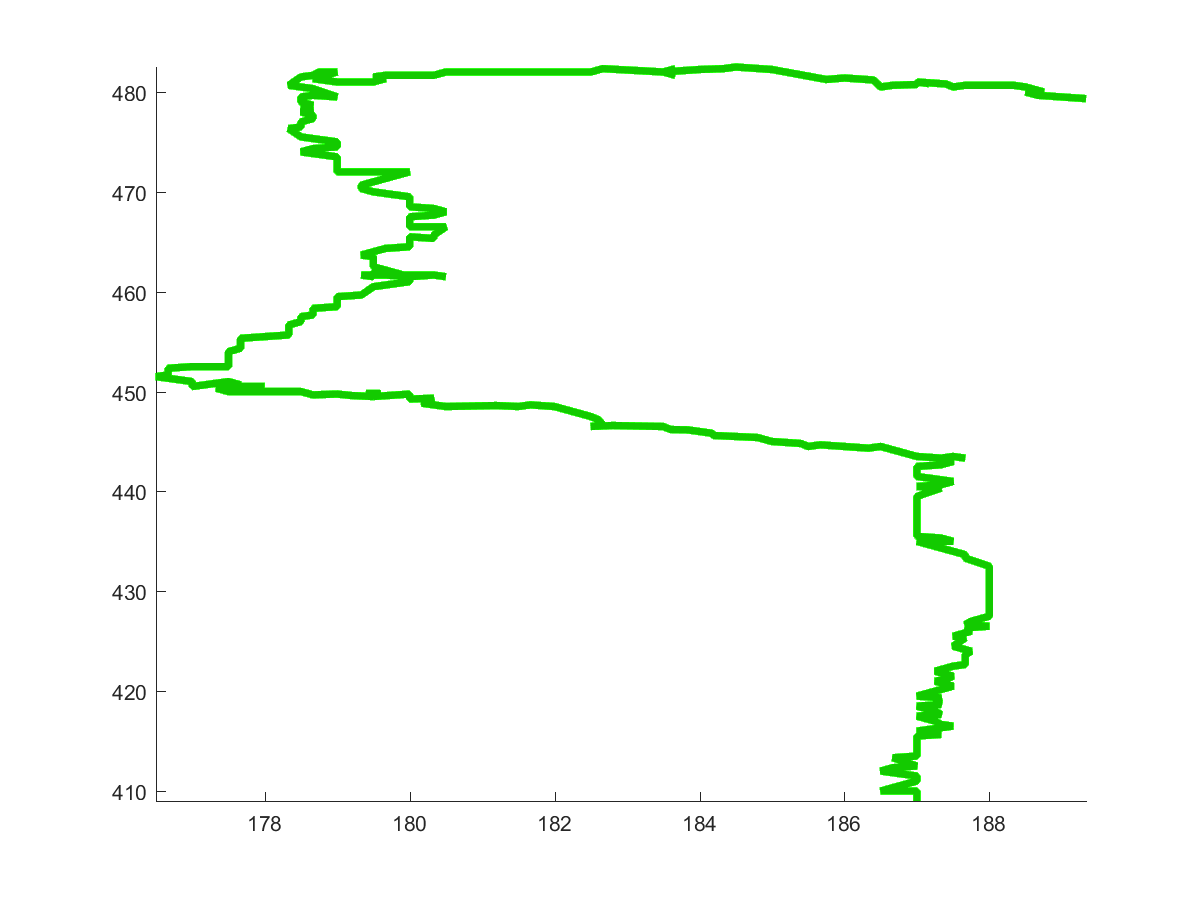
\includegraphics[width = 0.25\textwidth]{./images/bacteria/16.png}}\\
	\end{tabular}
	\caption{4 different tracked bacterial trajectories shown at $4$ different subsequent times. }
	\label{4traj}
\end{figure}
Due to the large number of particles often involved in such applications, a preliminary parallel GPGPU + MPI version of the framework is currently being developed which has provided promising results in terms of scalability and speed up, allowing much larger dataset to be analyzed. Eventually, it is worth to note that under the assumption of associativity of the \textit{assignment operator} $\lozenge$, the tracking algorithm could be implemented using the \textit{parallel reduction} design pattern.


